\documentclass{ubicomp2013}
\usepackage{times}
\usepackage{url}
\usepackage{graphics}
\usepackage{color}
\usepackage[pdftex]{hyperref}
\hypersetup{%
pdftitle={Your Title}, pdfauthor={Your Authors}, pdfkeywords={your
keywords}, bookmarksnumbered, pdfstartview={FitH}, colorlinks,
citecolor=black, filecolor=black, linkcolor=black, urlcolor=black,
breaklinks=true, }
\newcommand{\comment}[1]{}
\definecolor{Orange}{rgb}{1,0.5,0}
\newcommand{\todo}[1]{\textsf{\textbf{\textcolor{Orange}{[[#1]]}}}}

%\pagenumbering{arabic}  % Arabic page numbers for submission.  Remove this line to eliminate page numbers for the camera ready copy

\begin{document}
% to make various LaTeX processors do the right thing with page size
\special{papersize=8.5in,11in}
\setlength{\paperheight}{11in}
\setlength{\paperwidth}{8.5in}
\setlength{\pdfpageheight}{\paperheight}
\setlength{\pdfpagewidth}{\paperwidth}

% use this command to override the default ACM copyright statement
% (e.g. for preprints). Remove for camera ready copy.
%\toappear{Submitted for review to UbiComp 2013.}



\title{TUISLA: Wireless and Batteryless Phidgets \newline for Rapid Prototyping and Sensing}
\numberofauthors{2}
\author{
  \alignauthor First Author Name (Blank for Blind Review)\\
    \affaddr{Affiliation  (Blank for Blind Review)}\\
    \affaddr{Address  (Blank for Blind Review)}\\
    \email{e-mail address (Blank for Blind Review)}
 \alignauthor Second Author Name (Blank for Blind Review)\\
    \affaddr{Affiliation  (Blank for Blind Review)}\\
    \affaddr{Address  (Blank for Blind Review)}\\
    \email{e-mail address (Blank for Blind Review)}  }
\maketitle

\begin{abstract}
Most input devices are limited by communication and energy  
  
\end{abstract}

\keywords{Guides, instructions, authors' kit, conference publications.}

\category{H.5.2}{Information interfaces and presentation (e.g., HCI)}{Miscellaneous}.

\generalterms{This section is limited to the following 16 terms and
MUST be included on the first page of all submissions after the ACM
Categories section, then as well chosen properly on the Proceedings
or Publication's submission page: Algorithms, Design,
Documentation, Economics, Experimentation, Human Factors, Languages,
Legal Aspects, Management, Measurement, Performance, Reliability,
Security, Standardization, Theory, Verification.}

\section{Introduction}
Interactive  




\section{Related Work}


\subsection{Malleable computing}
all the projects related to VoodooIO and pushpin computing

http://comp.eprints.lancs.ac.uk/1552/1/2007-Malleable.pdf

http://resenv.media.mit.edu/classes/MAS965/readings/lifton02.pdf

Pin \& Play: The Surface as Network Medium

\subsection{Induction}
Paradiso early work

RFID sensors from this other MIT/Intel guy.

\subsection{RFID technology}
Marquadt

General explanation of rfid technology citing Roy want.


\section{TUISLA}

We provide here an overview of the system

\subsection{RFID based system}


\subsection{Abstract and Keywords}

Every submission should begin with an abstract of \textbf{no more than 150 words},
followed by a set of keywords. The abstract and keywords should be
placed in the left column of the first page under the left half of the
title. The abstract should be a concise statement of the problem,
approach and conclusions of the work described.  It should clearly
state the paper's contribution to the field of Ubiquitous Computing.

/*
\begin{figure}[t]
\begin{center}
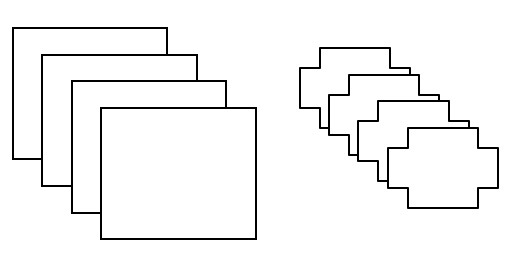
\includegraphics[width=0.90\columnwidth]{sample-fig.jpg}
\end{center}
\caption{Figure captions should be centered and placed below the
figure.}
\end{figure}
*/

The first set of keywords will be used to index the paper in the
proceedings. The second set are entries from the ACM Classification
System
%~\cite{acm_categories}, see\\
(http://www.acm.org/class/1998/), and used to catalogue the paper in the ACM
Digital Library.

\subsection{Normal or Body Text}

Please use a 10-point Times Roman font or, if this is unavailable,
another proportional font with serifs, as close as possible in
appearance to Times Roman 10-point. The Press 10-point font available
to users of Script is a good substitute for Times Roman. If Times
Roman is not available, try the font named Computer Modern Roman. On a
Macintosh, use the font named Times and not Times New Roman. Please
use sans-serif or non-proportional fonts only for special purposes,
such as headings or source code text.

\subsection{First Page Copyright Notice}

Include the copyright notice, as provided in this template, at the bottom of the left column of the first page.
\subsection{Subsequent Pages}

On pages beyond the first, start at the top of the page and continue
in double-column format.  The two columns on the last page should be
of equal length. Note the template provided for Latex users does not automatically balance columns at the end of the document. You will need to do this manually by inserting a page break, or use one of the additional packages available for this purpose (\emph{balance}, \emph{flushend}, or \emph{multicol}).

\subsection{References and Citations}

Use a numbered list of references at the end of the article, ordered
alphabetically by first author, and referenced by numbers in brackets, e.g.
``[2,4,5,7]". For papers from conference proceedings, include the title
of the paper and an abbreviated name of the conference (e.g., for
UbiComp 2008 proceedings, use Proc. UbiComp 2008). Do not include
the location of the conference or the exact date; do include the page
numbers if available. See the examples of citations at the end of this
document.

Your references should be published materials accessible to the
public.  Internal technical reports may be cited only if they are
easily accessible (i.e., you provide the address for obtaining the
report within your citation) and may be obtained by any reader for a
nominal fee.  Proprietary information may not be cited. Private
communications should be acknowledged in the main text, not referenced
(e.g., ``[Robertson, personal communication]'').


\section{Sections}
The heading of a section should be in Helvetica 9-point bold, all in capitals. Use Arial if Helvetica is not available. Sections should not be numbered.

\subsection{Subsections}
Headings of subsections should be in Helvetica 9-point bold with initial letters capitalized. (Note: For sub-sections and sub-subsections, a word like the or of is not capitalized unless it is the first word of the heading.)

\subsubsection{Sub-subsections}
Headings for sub-subsections should be in Helvetica 9-point italic with initial letters capitalized.

\section{Figures/Captions and optional Audio/Video}
Place figures and tables at the top or bottom of the appropriate column or columns, on the same page as the relevant text (see Figure 1). A figure or table may extend across both columns to a maximum width of 17.78 cm (7 in.).

Captions should be Times New Roman 9-point bold.  They should be numbered (e.g., ``Table 1" or ``Figure 2"), centered and placed beneath the figure or table.  Please note that the words ``Figure" and ``Table" should be spelled out (e.g., ``Figure" rather than ``Fig.") wherever they occur.

Papers and notes may use color figures, which are included in the page limit; the figures must be usable when printed in black and white in the proceedings.

You may provide up to two supporting audio or video files for your Full Paper or Note. However, the paper should stand on its own without this material, as it may not be available to everyone who reads the paper. Please note that your \textbf{total submission size cannot exceed 10.0 MB} (including your submission document and any additional material).

\subsection{Inserting Images}
To ensure that generated PDF Files are not larger than necessary, please resize and edit any images you include to an appropriate printing resolution (usually 600 dpi).

\subsection{Table Style}
There are various ways of producing tables in Latex. Generally, text in each field of a table will look better if it has equal amounts of spacing above and below it, as in Table 1.

\begin{table}[t]
\begin{center}
\begin{tabular}{|c|c|c|}
\hline
&&\\
{\bf Objects}   &   {\bf Caption pre-2002} & {\bf Caption since 2003}\\
&&\\
\hline
&&\\
Tables & Above & Below  \\
&&\\
\hline
&&\\
Figures & Below & Below  \\
&&\\
\hline
\end{tabular}
\caption{Table captions should be placed below the table.}
\end{center}
\end{table}



\section{Language, Style and Context}
The written and spoken language of the UbiComp conference is English. Spelling and punctuation may use any dialect of English (e.g., British, Canadian, US, etc.) provided this is done consistently. Hyphenation is optional. To ensure suitability for an international audience, please pay attention to the following:
\itemize
\item{Write in a straightforward style. }
\item{Try to avoid long or complex sentence structures. }
\item{Briefly define or explain all technical terms that may be unfamiliar to readers.}
\item{Explain all acronyms the first time they are used in your text � e.g., ``Digital Signal Processing (DSP)".}
\item{Explain local references (e.g., not everyone knows all city names in a particular country).}
\item{Explain ``insider" comments. Ensure that your whole audience understands any reference whose meaning you do not describe (e.g., do not assume that everyone has used a particular device or application).}
\item{Explain colloquial language and puns. Understanding phrases like ``red herring" may require a local knowledge of English.  Humor and irony are difficult to translate.}
\item{Use unambiguous forms for culturally localized concepts, such as times, dates, currencies and numbers (e.g., ``1-5- 97" or ``5/1/97" may mean 5 January or 1 May, and ``seven o{'}clock" may mean 7:00 am or 19:00).
%\item{Be careful with the use of gender-specific pronouns (he, she) and other gendered words (chairman, manpower, man-months). Use inclusive language that is gender-neutral (e.g., she or he, they, s/he, chair, staff, staff-hours, person-years). See \cite{schwartz95} for further advice and examples regarding gender and other personal attributes.}
\item{If possible, use the full (extended) alphabetic character set for names of persons, institutions, and places (e.g., Gr{\o}nb{\ae}k, Lafreni{\`e}re, S{\'a}nchez, Universit{\"a}t, Wei{\ss}enbach, Z{\"u}llighoven, {\AA}rhus, etc.).

\section{Page Numbering, Headers and Footers}
Please submit your anonymous version for reviewing with page numbers centered in the footer.  These must be removed in the final version of accepted papers, as page numbers, headers, and footers will be added by the conference printers. If you use the provided template, simply comment out \verb \pagenumbering{arabic} in the document header.

\section{Applications}
We recommend that you produce a PDF version of your submission well before the final deadline.  Besides making sure that you are able to produce a PDF, you will need to check that (a) the length of the file remains within the submission category's page limit (10 pages for Full Papers and 4 pages for Notes), (b) the PDF file size is 4 megabytes or less, and (c) the file can be read and printed using Adobe Acrobat Reader.

Test your PDF file by viewing or printing it with the same software we will use when we receive it, Adobe Acrobat Reader Version 9. This is widely available at no cost from~\cite{acrobat}.  Note that most reviewers will use a North American/European version of Acrobat reader, which cannot handle documents containing non-North American or non-European fonts (e.g., Asian fonts).  Please therefore do not use Asian fonts, and verify this by testing with a North American/European Acrobat reader (obtainable as above). Something as minor as including a space or punctuation character in a two-byte font can render a file unreadable.

\section{Discussion}

\section{Conclusion}

\section{Acknowledgements}


\bibliographystyle{abbrv}
\bibliography{tuisla}

\end{document}
